\documentclass[notes,color]{sepslide0}
\usepackage{graphicx}
\usepackage[overheads]{mysepslides}
\usepackage{tech,graphicx,url,csp-cm,tikz,scalalistings}

\title{Conditions and Targeted Signals} 
\author{Gavin Lowe}

% \everymath{\color{Plum}}
\def\smaller{\small} 
\def\scalacolour{\color{violet}}

\begin{document}

\begin{slide}
  
  \Title

\end{slide}


%% \begin{slide}
%% \heading{Multiple producers and consumers}

%% Recall the |Slot| example.
%% \begin{scala}
%% class Slot[T]{
%%   private var value = null.asInstanceOf[T]
%%   private var filled = false

%%   def put(v:T) = synchronized{
%%     while(filled) wait() // wait for the slot to be emptied
%%     value = v; filled = true; notify()
%%   }

%%   def get : T = synchronized{
%%     while(!filled) wait() // wait for the slot to be filled
%%     filled = false; notify(); value
%% } }
%% \end{scala}
%% This works correctly with a single producer and consumer, but not with
%% multiple ones. 
%% \end{slide}

%%%%%

%% \begin{slide}
%% \heading{Multiple producers and consumers}

%% Suppose we run the |Slot| with multiple producers and consumers.  It turns out
%% that we need to use |notifyAll| rather than |notify|.
%% %
%% Consider the following execution, if |notify| is used.
%% %
%% \begin{enumerate}
%% \item Two consumers run, and both have to wait.

%% \item Producer~1 runs, sets |filled = true|, wakes up consumer~1, and returns.

%% \item Producer~2 runs, but has to wait.

%% \item Consumer~1 runs, sets |filled = false|, calls |notify()| which wakes up
%% consumer~2, and returns.

%% \item Consumer~2 runs, finds |filled = false|, so waits again. 
%% \end{enumerate}
%% %
%% Now producer~2 and consumer~2 are both waiting, but they should have been able
%% to exchange data. 

%% If consumer~1 calls |notifyAll|, things will work correctly. 
%% \end{slide}

%%%%%

\begin{slide}
\heading{A slot for multiple producers and consumers}

Recall the |Slot| example, to be used by multiple producers and consumers,
implemented using a JVM monitor.
%
\begin{scala}
class Slot2[T]{
  private var value = null.asInstanceOf[T]
  private var filled = false

  def put(v:T) = synchronized{
    while(filled) wait()
    value = v; filled = true; notifyAll()
  }

  def get : T = synchronized{
    while(!filled) wait()
    filled = false; notifyAll(); value
  }
}
\end{scala}
\end{slide}

%%%%%

\begin{slide}
\heading{Targeted notifications}

The code on the previous slide isn't ideal: most threads that are awoken by a
|notifyAll| will be forced to wait again.

We would like to be able to target a |notify| by a |put| towards a thread
waiting in |get|; and target a |notify| by a |get| towards a thread
waiting in |put|.  This isn't possible using standard |notify|s.
\end{slide}

%%%%%

%% \begin{slide}
%% \heading{CSO monitors}

%% A CSO monitor is an extension of JVM monitors that allows more targeted
%% notifications.  

%% A new monitor is created with
%% \begin{scala}
%%   private val monitor = new Monitor
%% \end{scala}

%% The |withLock| method on monitors acts rather like a |synchronized| block:
%% \begin{scala}
%%   def put(v: T) = monitor.withLock{ ... }
%% \end{scala}  
%% At most one thread can be inside any |withLock| block on a given monitor.
%% \end{slide}

%%%%%

\begin{slide}
\heading{Conditions}

Signalling can be done via a |Condition|.  An SCL |Lock| can be
associated with any number of |Conditions|, created using the |newCondition|
operation.  For example
%
\begin{scala}
  private val lock = new Lock
  // Conditions for signalling the slot is empty or non-empty, respectively.
  private val empty = lock.newCondition
  private val nonEmpty = lock.newCondition
\end{scala}
%
(Choose good names for your conditions, and write comments to make clear their
roles.)
\end{slide}

%%%%%

\begin{slide}
\heading{Conditions}

Each condition has operations as follows:
%
\begin{itemize}
\item |await()|: wait for a signal on this condition;
\item |signal()|: signal to a thread waiting on this condition;
\item |signalAll()|: signal to all threads waiting on this condition.
\end{itemize}
%
Each operation should be performed while holding the related lock. 

An |await| releases the lock.  When it receives a signal, it has to re-obtain
the lock before proceeding.

We can implement monitors using |Lock|s and |Condition|s. 
\end{slide}

%%%%%

\begin{slide}
\heading{The slot, using conditions}

\begin{scala}
class MonitorSlot[T]{
  private var value = null.asInstanceOf[T]
  private var filled = false
  private val lock = new Lock
  // conditions for signalling the slot is empty or non-empty, respectively.
  private val empty, nonEmpty = lock.newCondition

  def put(v: T) = lock.mutex{
    while(filled) empty.await()           // wait for the slot to be emptied (1)
    value = v; filled = true; nonEmpty.signal() // signal to a get at (2)
  }

  def get: T = lock.mutex{
    while(!filled) nonEmpty.await()     // wait for the slot to be filled (2)
    filled = false; empty.signal()        // signal to a put at (1)
    value
} }
\end{scala}
\end{slide}

%%%%%
{\advance \slideheight by 2mm
\begin{slide}
\heading{Waiting for a condition}

It is often useful to wait on a |Condition| until some test becomes true.  The
following operation on a |Condition| provides this.
\begin{scala}
  def await(test: => Boolean): Unit = while(!test) await()
\end{scala}

For example
%
\begin{scala}
  def put(v: T) = lock.mutex{
    empty.await(!filled)                  // wait for the slot to be emptied (1)
    value = v; filled = true; nonEmpty.signal() // signal to a get at (2)
  }

  def get: T = lock.mutex{
    nonEmpty.await(filled)               // wait for the slot to be filled (2)
    filled = false; empty.signal()       // signal to a put at (1)
    value
  }
\end{scala}
\end{slide}}

%%%%%

\begin{slide}
\heading{Spurious wake-ups}

The implementation of SCL |Condition|s protects against spurious
wake-ups: a waiting thread will wake up \emph{only} when another
thread sends a signal.  (The same is not true of the implementation in
\texttt{java.util.concurrent.locks.Condition}!)

However, it might sometimes be necessary to re-check the relevant
condition after an |await|, in case another thread has invalidated it.
For example, on the previous slide, a waiting |get| may receive a
signal from a |put|; but another |get| may take the deposited value
before the first |get| obtains the lock.
\end{slide}

%%%%%

\begin{slide}
\heading{JVM monitors versus SCL monitors}

SCL monitors are convenient when one wants to target signals.
However, their implementation is more expensive than JVM monitors: use
SCL monitors only when there is a good reason to do so.
\end{slide}


%%%%%%%%%%%%%%%%%%%%%%%%%%%%%%%%%%%%%%%%%%%%%%%%%%%%%%%%%%%%

\begin{slide}
\heading{A bounded partial queue}

Concurrent datatypes can be implemented using monitors. 

We will implement a bounded partial queue.
%
\begin{itemize}
\item |dequeue| operations will block while the queue is empty;

\item |enqueue| operations will block while the queue is full.
\end{itemize}
\end{slide}

%%%%%

\begin{slide}
\heading{A bounded partial queue}

\begin{scala}
/** A bounded partial queue implemented as a monitor. */
class BoundedMonitorPartialQueue[T](bound: Int) extends PartialQueue[T]{
  /** The queue itself. */
  private val queue = new scala.collection.mutable.Queue[T]

  /** A lock, to control the synchronisations. */
  private val lock = new Lock

  /** Condition for signalling that the queue is not full. */
  private val notFull = lock.newCondition

  /** Condition for signalling that the queue is not empty. */
  private val notEmpty = lock.newCondition
  ...
}
\end{scala}
\end{slide}

%%%%%

\begin{slide}
\heading{A bounded partial queue}

\begin{scala}
  /** Enqueue x.  Blocks until the queue is not full. */
  def enqueue(x: T) = lock.mutex{
    notFull.await(queue.length < bound)           // wait for a signal (1)
    queue.enqueue(x); notEmpty.signal()           // signal to a dequeue at (2)
  }

  /** Dequeue a value.  Blocks until the queue is non-empty. */
  def dequeue: T = lock.mutex{
    notEmpty.await(queue.nonEmpty)               // wait for a signal (2)
    val result = queue.dequeue; notFull.signal()  // signal to an enqueue at (1)
    result
  }
\end{scala}
\end{slide}


  % /** Shut down the queue. */
  % def shutdown = {} // nothing needs doing

\begin{slide}
\heading{A synchronous channel}

We will implement a synchronous channel, for use by an arbitrary number of
senders and receivers.  

We will require three signals between threads:
%
\begin{itemize}
\item Each sender will signal to a receiver that it has deposited a value,
  which the receiver can take;

\item The receiver will then signal back to the sender that it can continue;
  this makes the channel synchronous;

\item The receiver will signal to a sender for the next round that it has
  cleared the value, so that sender can deposit its value.
\end{itemize}
%
We will use a separate condition for each signal. 
\end{slide}

%%%%%

\begin{slide}
\heading{A synchronous channel}

\begin{scala}
class SharedSyncChan[A]{
  /** The current or previous value. */
  private var value = null.asInstanceOf[A]

  /** Is the current value of value valid, i.e. ready to be received? */
  private var full = false
  ...
}
\end{scala}
\end{slide}

%%%%%

\begin{slide}
\heading{A synchronous channel}

\begin{scala}
  /** Lock for controlling synchronisations. */
  private val lock = new Lock

  /** Condition for signalling to receiver that a value has been 
    * deposited. */
  private val slotFull = lock.newCondition

  /** Condition for signalling to current sender that it can continue. */
  private val continue = lock.newCondition

  /** Condition for signalling to the next sender that the previous value 
    * has been read. */
  private val slotEmptied = lock.newCondition
\end{scala}
\end{slide}

%%%%%

\begin{slide}
\heading{A synchronous channel}

\begin{scala}
  def send(x: A) = lock.mutex{
    slotEmptied.await(!full)  // wait for previous value to be consumed (1)
    value = x; full = true   // deposit my value
    slotFull.signal()         // signal to receiver at (2)
    continue.await()          // wait for receiver (3)
  }

  def receive: A = lock.mutex{
    slotFull.await(full)     // wait for sender (2)
    continue.signal()        // signal to current sender at (3) 
    full = false             // clear value
    slotEmptied.signal()     // signal to next sender at (1)
    value
  }
\end{scala}
\end{slide}

%%%%%

\begin{slide}
\heading{A synchronous channel}

Note that is necessary for the sender to recheck |full| when it receives a
signal on |slotEmptied|, in case another sender has run in the meantime and
filled the slot.

Likewise with the receiver on |slotFull|.

However, there is no need for the sender to perform a similar check on
receiving a signal on |continue|, because it cannot be preempted by another
sender. 
\end{slide}

%%%%%

\begin{slide}
\heading{Testing}

We can test this implementation by running some threads that perform sends and
receives, and have them logging the call and return of each operation.  For
simplicity, we arrange that every send is of a different value.  This makes it
easy to identify matching sends and receives (if they exist).  We then check
that the two invocations overlap.

It is sound to assume the values sent are all different, because the
implementation is \emph{data independent} in the type |A| of data: values of
this type are stored, read, and returned, but no operation (e.g.~|==|) is
done on them.  This means that for any erroneous history, there would be a
corresponding erroneous history using distinct values.
\end{slide}
 % many-many channel
% The following example should be adapted to use Monitors/QueueM.  However,
% the example makes more sense using semaphores, s0 let's leave it out. 
%
\begin{slide}
\heading{Example: a monitor to enforce mutual exclusion}

Often client processes need to access a shared resource under \emph{mutual
  exclusion}: only one client may use the resource at a time.  We will
implement a monitor to enforce mutual exclusion, but also to allow clients
to access the resource in first-come-first-served order.  

When a client wishes to access the resource it calls a \SCALA{Request}
procedure (known as the \emph{entry protocol}), passing in its identity; this
will block until this client is allowed access.  After using the resource, the
client calls a \SCALA{Release} procedure (known as the \emph{exit protocol}).
So the code for a client will look like
%
\begin{scala}
...
Monitor.Request(me) // entry protocol
...                  // use resource
Monitor.Release     // exit protocol
...
\end{scala}
\end{slide}

%%%%%

\begin{slide}
\heading{First attempt}

The following version enforces mutual exclusion, but not FIFO behaviour.
%
\begin{scala}
object Monitor{
  private var busy = false // Is the resource in use?

  def Request(id: ProcId) = synchronized{
    while(busy) wait() // wait turn
    busy = true
  }

  def Release = synchronized{
      busy = false
      notify()
  }
}
\end{scala}
\end{slide}

%%%%%

\begin{slide}
\heading{Enforcing FIFO}

We use a queue to store the identities of waiting processes:
%
\begin{scala}
val queue = new scala.collection.mutable.Queue[ProcId];
\end{scala}

If a process cannot access the resource immediately, its identity is put on
the queue and it waits.  When it is woken up, it checks whether it has got to
the front of the queue.
%
\begin{scala}
def Request(id: ProcId) = synchronized{
  if(busy || !queue.isEmpty){
    queue.enqueue(id);
    while(busy || queue.first!=id) wait(); // wait turn
    val first = queue.dequeue;
    assert(first==id);
  }
  busy = true;
}
\end{scala}
\end{slide}

%%%%%

\begin{slide}
\heading{Enforcing FIFO}

The \SCALA{Release} method is as before.

If processes do not have identities, the monitor can give each process a
unique sequence number to act as its identity:
%
\begin{scala}
private var next = 0; // next sequence number to use

def Request = synchronized{
  val id = next; next += 1;
  ... // as before
}
\end{scala}
\end{slide}


\begin{slide}
\heading{The sleeping barber}

Different concurrent programs produce different synchronisation problems.
Often these are presented in terms of colourful real-life scenarios.  One such
example is the sleeping barber.

A small barbershop is run by a single barber, and has several chairs.  When
there are no customers, the barber sleeps in his chair.  When a customer
arrives and finds the barber sleeping, he wakes up the barber, sits in the
chair, and sleeps while the barber cuts his hair.  If another customer arrives
in the meantime, he sleeps in one of the other chairs.  When the barber
finishes the haircut, he wakes up the customer, and holds the door open and
waits for him to leave.  If there are waiting customers, he wakes one up and
waits for him to sit in the chair; otherwise, he goes back to sleep.
\end{slide}

%%%%%

\begin{slide}
\heading{The sleeping barber}

We will implement a monitor to solve this synchronization problem.  The
monitor will have the following methods:
%
\begin{description}
\item[getNextCustomer]
The barber wakes up a customer and waits for him to sit in the chair, or
sleeps until a customer arrives;

\item[getHaircut]
A customer arrives and waits until the barber is ready, then sits in the
chair;

\item[finishedCut]
The barber wakes up the customer, and waits for him to leave;

\item[waitForHaircut]
The customer waits for the barber to finish, then leaves.
\end{description}
%
Each pair of methods will involve a signal in each direction between the two
parties.
\end{slide}

\begin{slide}
\heading{Barber and customer processes}

The barber and customer processes must call the appropriate methods in order;
for example:
%
\begin{scala}
  def barber = thread("Barber"){
    while(true){
      sleep(Random.nextInt(500)); println("Barber ready")
      Barber.getNextCustomer; println("Barber cutting hair")
      sleep(Random.nextInt(500)+1000); println("Barber finished")
      Barber.finishedCut
  } }

  def customer(me: Int) = thread("Customer"+me){
    while(true){
      sleep(Random.nextInt(6000)); println("Customer "+me+" arrived")
      Barber.getHaircut; println("Customer "+me+" getting haircut")
      Barber.waitForHaircut; println("Customer "+me+" finished haircut")
  } }
\end{scala}
\end{slide}

%%%%%

\begin{slide}
\heading{Variables and conditions}

Each procedure will involve signalling to the other party.  We include a
condition for each signal.  However, in two cases it's possible that the
signal is sent before the other party is waiting for it; we use boolean
variables to cover these cases.

\begin{scala}
object Barber{
  /** Is the barber ready to cut hair, or finished the last cutting? */
  private var barberAvailable = false; private var barberDone = false

  private val lock = new Lock
  
  /** Conditions to signal that the barber is ready, the customer is ready,
    * the barber has finished cutting, and the customer has left. */
  private val barberAvailableC, chairOccupiedC, barberDoneC, customerLeftC =
    lock.newCondition
  ...
}
\end{scala}
\end{slide}

%%%%%

\begin{slide}
\heading{Sequence diagram}

\def\cx{4.0} \def\ba{8.5} \def\bd{11.5}
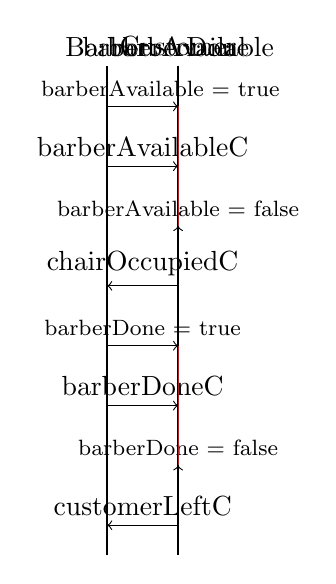
\begin{tikzpicture}[yscale = 0.76,xscale = 0.9]
\draw(0,0) node (b) {Barber};
\draw[black,thick] (b) -- ++ (0,-8.5);
\draw(\cx,0) node (c) {Customer};
\draw[black,thick] (c) -- ++ (0,-8.5);
\draw(\ba,0) node (ba) {\scalashape barberAvailable};
\draw(\bd,0) node (bd) {\scalashape barberDone};
%
\draw[->] (0,-1) -- 
  node[above,near end]{\footnotesize\scalashape barberAvailable = true}
  (\ba,-1);
\draw[->] (0,-2) -- node[above]{\scalashape barberAvailableC} (\cx,-2);
\draw[->] (\cx,-3) -- 
  node[above]{\footnotesize\scalashape barberAvailable = false}
  (\ba,-3);
\draw[red] (\ba,-1) -- (\ba,-3);
\draw[<-] (0,-4) -- node[above]{\scalashape chairOccupiedC} (\cx,-4);
%
\draw[->] (0,-5) -- node[above]{\footnotesize\scalashape barberDone = true}
   (\bd,-5);
\draw[->] (0,-6) -- node[above]{\scalashape barberDoneC} (\cx,-6);
\draw[->] (\cx,-7) -- node[above]{\footnotesize\scalashape barberDone = false}
   (\bd,-7);
\draw[red] (\bd,-5) -- (\bd,-7);
\draw[<-] (0,-8) -- node[above]{\scalashape customerLeftC} (\cx,-8);

\end{tikzpicture}
\end{slide}

%%%%%

\begin{slide}
\heading{The first two signals}

The barber signals that he is ready using |barberAvailableC|.  However, a
customer might not have arrived yet, so he also sets |barberAvailable|.  The
customer has to recheck |barberAvailable| when he awakes, in case another
customer has arrived and taken the slot. 

The barber then waits for a signal on |chairOccupiedC|.  There is only one
barber, and he must be waiting before the signal is sent, so nothing more is
needed. 
\end{slide}

%%%%%

\begin{slide}
\heading{The first two signals}

\begin{scala}
  /** Barber waits for next customer. */
  def getNextCustomer = lock.mutex{
    barberAvailable = true
    barberAvailableC.signal()                  // signal to a customer at (1)
    chairOccupiedC.await()                     // wait for signal (2)
  }

  /** Customer waits for barber to be available. */ 
  def getHaircut = lock.mutex{
    barberAvailableC.await(barberAvailable) // wait for barber (1)
    barberAvailable = false                   // clear for next round
    chairOccupiedC.signal()                   // signal to barber at (2)
  }
\end{scala}
\end{slide}

%%%%%

\begin{slide}
\heading{The third and fourth signals}

The barber signals he has finished on |barberDoneC|.  However, it's possible that
the customer isn't yet waiting, so he also sets |barberDone|.  No other
customer can be waiting on this signal, so nothing more is needed.

The barber then waits for a signal on |customerLeftC|.  Again he must be
waiting before the signal is sent, so nothing more is needed.
\begin{scala}
  def finishedCut = lock.mutex{
    barberDone = true; barberDoneC.signal()  // wake up customer at (3)
    customerLeftC.await()                        // wait for customer to leave (4)
  }

  def waitForHaircut = lock.mutex{
    if(!barberDone) barberDoneC.await()     // wait for barber to finish (3)
    assert(barberDone); barberDone = false  // clear for next round
    customerLeftC.signal()                     // signal to barber at (4)
  }
\end{scala}
\end{slide}




%%%%%
%%%%%%%%%%%%%%%%%%%%%%%%%%%%%%%%%%%%%%%%%%%%%%%%%%%%%%%
% \begin{slide}
% \heading{The status of the scenario}

% The scenario has four stages: the barber waiting for a customer; the customer
% sitting in the chair getting a haircut; the barber waiting for the customer to
% leave; the customer having left.   We therefore have a variable that records
% the current status:
% %
% \begin{scala}
% val barberAvailable = 0; 
% val chairOccupied = 1; 
% val doorOpen = 2; 
% val customerLeft = 3;
% var status = -1;
% \end{scala}
% \end{slide}

% %%%%%

% \begin{slide}
% \heading{The first two stages}

% The barber signals to a sleeping customer (if any), and waits until the chair
% is occupied.  The customer waits for the barber to be ready, occupies the
% chair, and signals to the barber.
% %
% \begin{scala}
% def GetNextCustomer = synchronized{
%   status = barberAvailable;
%   notify(); // wake up a sleeping customer
%   while(status!=chairOccupied) wait(); // wait for customer
% }

% def GetHaircut = synchronized{
%   while(status!=barberAvailable) wait(); // wait for barber
%   status = chairOccupied;
%   notifyAll(); // Signal to barber
% }
% \end{scala}
% \end{slide}

% %%%%%

% \begin{slide}
% \heading{The last two stages}

% The barber opens the door, signals to the customer, and waits for the customer
% to leave.  The customer waits for the barber to open the door, leaves, and
% signals to the barber.
% %
% \begin{scala}
% def FinishedCut = synchronized{
%   status = doorOpen;
%   notifyAll(); // signal to customer
%   while(status!=customerLeft) wait(); 
%     // wait for customer to leave
% }

% def WaitForHaircut = synchronized{
%   while(status!=doorOpen) wait(); // wait for barber to finish
%   status = customerLeft; 
%   notifyAll(); // Signal to barber
% }
% \end{scala}
% \end{slide}

% %%%%%

% \begin{selfnote}
% Note use of \SCALA{notifyAll()}

% Moral: identify the scenarios under which processes might be woken up; use
% state variables to ensure that processes wake up only under the appropriate
% circumstances, and only the appropriate number are woken up. 
% \end{selfnote}

%%%%%

\begin{slide}
\heading{Synchronisation problems}

Synchronisation problems like this can be difficult.  In order to come up with
a correct and understandable design, it is useful to use state variables that
indicate which processes are in different states, at least in \emph{quiescent
  states} when no processes
are running or runnable.

For example, the |barberAvailable| variable records (in quiescent states) that
the barber is waiting for a signal in |getNextCustomer|.  The customer that
will be served next clears this variable before signalling to the barber and
releasing the lock.

The |barberDone| variable records (in quiescent states) that the barber is
waiting for a signal in |finishedCut|.  The current customer clears this
variable before signalling to the barber and releasing the lock.
\end{slide}

%%%%%

% {\advance\slideheight by 3mm
% \begin{slide}
% \heading{Synchronisation problems}

% For example, with the sleeping barber, when no processes are running or
% runnable:
% %
% \begin{itemize}
% \item
% If \SCALA{barberAvailable = true} then the barber is waiting in
% \SCALA{GetNextCustomer} and no customers are in the module;

% \item
% If \SCALA{status == chairOccupied} then the barber is not in the module, one
% customer might be waiting in \SCALA{WaitForHaircut} (or has finished
% \SCALA{GetHairCut} and not yet started \SCALA{WaitForHairCut}), and other
% customers might be waiting in \SCALA{GetHairCut}.
% \end{itemize}
% %
% And
% %
% \begin{itemize}
% \item
% If \SCALA{status == doorOpen} then the barber is waiting in
% \SCALA{FinishedCut}, one customer is running or runnable in
% \SCALA{WaitForHairCut}, and other customers might be waiting in
% \SCALA{GetHairCut};

% \item
% If \SCALA{status == customerLeft} then the barber is running or runnable in
% \SCALA{FinishedCut}, or has exited \SCALA{FinishedCut}.
% \end{itemize}
% \end{slide}}

%%%%%

\begin{slide}
\heading{Synchronisation problems}

In other synchronisation problems, it can be useful to keep track of:
%
\begin{itemize}
\item 
How many processes are waiting in various waits;

\item
How many processes have completed operations (or maybe the difference between
the number of times two matching operations have been completed).
\end{itemize}

To track down bugs, it can be useful to:
\begin{itemize}
\item write lots of assertions;

\item use logging, particularly of the sending and receiving of
signals.
\end{itemize}
\end{slide}


%%%%%

\begin{slide}
\heading{Other languages}

Most other languages provide a mechanism similar to conditions.  For example
%
\begin{itemize}
\item Implementations of the Java interface
  |java.util.concurrent.locks.Condition|;

\item C++ |condition_variable|s.
\end{itemize}
%
Note that both of the above may suffer from spurious wake-ups.
\end{slide}

%%%%%

\begin{slide}
\heading{Summary}

\begin{itemize}
\item Conditions and targeted signals;

\item Examples;

\item Dealing with synchronisation problems.
\end{itemize}
\end{slide}


\end{document}
